%%%%%%%%%%%%%%%%%%%%%%%%%%%%%%%%%%%%%%%%%
% Beamer Presentation
% LaTeX Template
% Version 1.0 (10/11/12)
%
% This template has been downloaded from:
% http://www.LaTeXTemplates.com
%
% License:
% CC BY-NC-SA 3.0 (http://creativecommons.org/licenses/by-nc-sa/3.0/)
%
%%%%%%%%%%%%%%%%%%%%%%%%%%%%%%%%%%%%%%%%%

%----------------------------------------------------------------------------------------
%	PACKAGES AND THEMES
%----------------------------------------------------------------------------------------

\documentclass{beamer}

\mode<presentation> {

% The Beamer class comes with a number of default slide themes
% which change the colors and layouts of slides. Below this is a list
% of all the themes, uncomment each in turn to see what they look like.

%\usetheme{default}
%\usetheme{AnnArbor}
%\usetheme{Antibes}
%\usetheme{Bergen}
%\usetheme{Berkeley}
%\usetheme{Berlin}
%\usetheme{Boadilla}
%\usetheme{CambridgeUS}
%\usetheme{Copenhagen}
%\usetheme{Darmstadt}
%\usetheme{Dresden}
%\usetheme{Frankfurt}
%\usetheme{Goettingen}
%\usetheme{Hannover}
%\usetheme{Ilmenau}
%\usetheme{JuanLesPins}
%\usetheme{Luebeck}
\usetheme{Madrid}
%\usetheme{Malmoe}
%\usetheme{Marburg}
%\usetheme{Montpellier}
%\usetheme{PaloAlto}
%\usetheme{Pittsburgh}
%\usetheme{Rochester}
%\usetheme{Singapore}
%\usetheme{Szeged}
%\usetheme{Warsaw}

% As well as themes, the Beamer class has a number of color themes
% for any slide theme. Uncomment each of these in turn to see how it
% changes the colors of your current slide theme.

%\usecolortheme{albatross}
%\usecolortheme{beaver}
%\usecolortheme{beetle}
%\usecolortheme{crane}
%\usecolortheme{dolphin}
%\usecolortheme{dove}
%\usecolortheme{fly}
%\usecolortheme{lily}
%\usecolortheme{orchid}
%\usecolortheme{rose}
%\usecolortheme{seagull}
%\usecolortheme{seahorse}
\usecolortheme{whale}
%\usecolortheme{wolverine}

\setbeamertemplate{footline} % To remove the footer line in all slides uncomment this line
%\setbeamertemplate{footline}[page number] % To replace the footer line in all slides with a simple slide count uncomment this line

\setbeamertemplate{navigation symbols}{} % To remove the navigation symbols from the bottom of all slides uncomment this line

}

\usepackage{graphicx} % Allows including images
\usepackage{booktabs} % Allows the use of \toprule, \midrule and \bottomrule in tables
\usepackage{sansmathaccent}
\pdfmapfile{+sansmathaccent.map}

\usepackage{tikz}
\usetikzlibrary{arrows, trees}
%----------------------------------------------------------------------------------------
%	TITLE PAGE
%----------------------------------------------------------------------------------------

\title[Algorithms 2]{Greedy Algorithms 2} % The short title appears at the bottom of every slide, the full title is only on the title page

%\author{John Smith} % Your name
\institute[BYU] % Your institution as it will appear on the bottom of every slide, may be shorthand to save space
{
Brigham Young University \\ % Your institution for the title page
\medskip
%\textit{john@smith.com} % Your email address
}
\date{\today} % Date, can be changed to a custom date

\begin{document}

\begin{frame}
\titlepage % Print the title page as the first slide
\end{frame}

%\begin{frame}
%\frametitle{Overview} % Table of contents slide, comment this block out to remove it
%\tableofcontents % Throughout your presentation, if you choose to use \section{} and %\subsection{} commands, these will automatically be printed on this slide as an overview of your presentation
%\end{frame}

%----------------------------------------------------------------------------------------
%	PRESENTATION SLIDES
%----------------------------------------------------------------------------------------

%------------------------------------------------
%\section{First Section} % Sections can be created in order to organize your presentation into %discrete blocks, all sections and subsections are automatically printed in the table of contents %as an overview of the talk
%------------------------------------------------

%\subsection{Subsection Example} % A subsection can be created just before a set of slides with %a common theme to further break down your presentation into chunks

%\begin{frame}
%\frametitle{AVL trees}
%Sed iaculis dapibus gravida. Morbi sed tortor erat, nec interdum arcu. Sed id lorem lectus. %Quisque viverra augue id sem ornare non aliquam nibh tristique. Aenean in ligula nisl. Nulla sed %tellus ipsum. Donec vestibulum ligula non lorem vulputate fermentum accumsan neque mollis.%\\~\\

%Sed diam enim, sagittis nec condimentum sit amet, ullamcorper sit amet libero. Aliquam vel dui %orci, a porta odio. Nullam id suscipit ipsum. Aenean lobortis commodo sem, ut commodo leo %gravida vitae. Pellentesque vehicula ante iaculis arcu pretium rutrum eget sit amet purus. %Integer ornare nulla quis neque ultrices lobortis. Vestibulum ultrices tincidunt libero, quis %commodo erat ullamcorper id.
%\end{frame}

%---------------------------------------------
%Dijkstra
\begin{frame}
\frametitle{Dijkstra's Algorithm}

\begin{itemize}
\item Finds the shortest paths from one node to all others.
\item Similar to Prim's algorithm.
\end{itemize}

\end{frame}
%---------------------------------------------------
\begin{frame}
\frametitle{Dijkstra's Algorithm}
\begin{itemize}
\item Start with a dictionary $d$ that takes a node to its distance from the starting node.
\item Mark the node with the shortest distance and add it to the tree.
\item Update distances.
\end{itemize}
\end{frame}
%-----------------------------------------------------
\begin{frame}
\frametitle{Dijkstra Example}

\begin{columns}[c]
\column{.5\textwidth}
\[
\begin{tabular}{|c|c|c|c|c|c|}
\hline
A\only<2->{*}&B&C&D&E&F \\
\hline
\only<2->{0}& ~&~ &~ &~&~\\
\hline
\only<3>{0}& \only<3>{2}&~ &\only<3>{5} &~&~\\
\hline
~& ~&~ &~ &~&~\\
\hline
~& ~&~ &~ &~&~\\
\hline
~& ~&~ &~ &~&~\\
\hline
~& ~&~ &~ &~&~\\
\hline
~& ~&~ &~ &~&~\\
\hline
\end{tabular}
\]

\begin{itemize}
\only<1-2>{\item Start at $A$}
\only<3>{\item Update A's neighbor's distances}
\end{itemize}

\column{.5\textwidth}

\begin{center}
\begin{tikzpicture}[->,>=stealth',auto,node distance=1.5cm,
 thick,main node/.style={circle,draw}]
 \only<1>{\node[main node](A)[]{A};}
 \only<2->{\node[main node,fill=blue!40!cyan](A)[]{A};}
 \node[main node](D)[right of = A]{D};
 \foreach \s/\t in {B/A, E/D, C/B, F/E}{ 
     \node[main node](\s)[below of = \t]{\s};}

\only<1>{ \path[every node/.style={font=\small}]
    (A) edge node{5} (D)
         edge node[left]{2} (B);}

\only<2->{ \path[every node/.style={font=\small}, blue!40!cyan]
    (A) edge node{5} (D)
         edge node[left]{2} (B);}

 \path[every node/.style={font=\small}]
    (B) edge node[below]{2} (D)
         edge node[below]{7} (E)
         edge node [left]{9} (F)
         edge node[left]{5} (C)
    (C) edge node[below]{2} (F)
    (D) edge node{4} (E)
    (E) edge node{3} (F);
 \end{tikzpicture}
 \end{center}
\end{columns}

\end{frame}
%-----------------------------------------------------
\begin{frame}
\frametitle{Dijkstra Example}

\begin{columns}[c]
\column{.5\textwidth}
\[
\begin{tabular}{|c|c|c|c|c|c|}
\hline
A*&B*&C&D&E&F \\
\hline
0& ~&~ &~ &~&~\\
\hline
0&2&~ &5&~&~\\
\hline
0&2&\only<2>{7}&\only<2>{4}&\only<2>{9}&\only<2>{11}\\
\hline
~& ~&~ &~ &~&~\\
\hline
~& ~&~ &~ &~&~\\
\hline
~& ~&~ &~ &~&~\\
\hline
~& ~&~ &~ &~&~\\
\hline
\end{tabular}
\]

\begin{itemize}
\only<1>{\item Add the node with the shortest distance}
\only<2->{\item Update B's neighbor's distances}
\end{itemize}

\column{.5\textwidth}
\begin{center}
\begin{tikzpicture}[->,>=stealth',auto,node distance=1.5cm,
 thick,main node/.style={circle,draw}]
\node[main node,fill=blue!40!cyan](A)[]{A};
 \node[main node](D)[right of = A]{D};
 \foreach \s/\t in {B/A}{ 
     \node[main node, fill=blue!40!cyan](\s)[below of = \t]{\s};}
 \foreach \s/\t in {E/D, C/B, F/E}{ 
     \node[main node](\s)[below of = \t]{\s};}

\only<1>{
  \path[every node/.style={font=\small},blue!40!cyan]
   (A) edge node{5} (D)
         edge node[left]{2} (B);
  \path[every node/.style={font=\small}]
   (B) edge node[below]{2} (D)
         edge node[below]{7} (E)
         edge node [left]{9} (F)
         edge node[left]{5} (C);
}
         
\only<2>{
 \path[every node/.style={font=\small},blue!40!cyan]
   (A) edge node[left]{2} (B)
    (B) edge node[below]{2} (D)
         edge node[below]{7} (E)
         edge node [left]{9} (F)
         edge node[left]{5} (C);
  \path[every node/.style={font=\small}]
    (A) edge node{5} (D);
}
 \path[every node/.style={font=\small}]
    (C) edge node[below]{2} (F)
    (D) edge node{4} (E)
    (E) edge node{3} (F);
 \end{tikzpicture}
 \end{center}
\end{columns}

\end{frame}
%-----------------------------------------------------
\begin{frame}
\frametitle{Dijkstra Example}

\begin{columns}[c]
\column{.5\textwidth}
\[
\begin{tabular}{|c|c|c|c|c|c|}
\hline
A*&B*&C&D*&E&F \\
\hline
0& ~&~ &~ &~&~\\
\hline
0&2&~ &5&~&~\\
\hline
0&2&7&4&9&11\\
\hline
0& 2&\only<2>{7}&4&\only<2>{8}&\only<2>{11}\\
\hline
~& ~&~ &~ &~&~\\
\hline
~& ~&~ &~ &~&~\\
\hline
~& ~&~ &~ &~&~\\
\hline
\end{tabular}
\]

\begin{itemize}
\only<1>{\item Add the node with the shortest distance}
\only<2->{\item Update D's neighbor's distances}
\end{itemize}

\column{.5\textwidth}
\begin{center}
\begin{tikzpicture}[->,>=stealth',auto,node distance=1.5cm,
 thick,main node/.style={circle,draw}]
\node[main node,fill=blue!40!cyan](A)[]{A};
 \node[main node,fill=blue!40!cyan](D)[right of = A]{D};
 \foreach \s/\t in {B/A}{ 
     \node[main node, fill=blue!40!cyan](\s)[below of = \t]{\s};}
 \foreach \s/\t in {E/D, C/B, F/E}{ 
     \node[main node](\s)[below of = \t]{\s};}

\only<1>{
 \path[every node/.style={font=\small},blue!40!cyan]
   (A) edge node[left]{2} (B)
    (B) edge node[below]{2} (D)
         edge node[below]{7} (E)
         edge node [left]{9} (F)
         edge node[left]{5} (C);
  \path[every node/.style={font=\small}]
    (A) edge node{5} (D)
    (D) edge node{4} (E);
}
\only<2>{
 \path[every node/.style={font=\small},blue!40!cyan]
   (A) edge node[left]{2} (B)
    (B) edge node[below]{2} (D)
         edge node [left]{9} (F)
         edge node[left]{5} (C)
    (D) edge node{4} (E);
  \path[every node/.style={font=\small}]
    (A) edge node{5} (D)
    (B) edge node[below]{7} (E);
}

 \path[every node/.style={font=\small}]
    (C) edge node[below]{2} (F)
    (E) edge node{3} (F);
 \end{tikzpicture}
 \end{center}
\end{columns}

\end{frame}
%-----------------------------------------------------
\begin{frame}
\frametitle{Dijkstra Example}

\begin{columns}[c]
\column{.5\textwidth}
\[
\begin{tabular}{|c|c|c|c|c|c|}
\hline
A*&B*&C*&D*&E&F \\
\hline
0& ~&~ &~ &~&~\\
\hline
0&2&~ &5&~&~\\
\hline
0&2&7&4&9&11\\
\hline
0& 2&7&4&8&11\\
\hline
0& 2&7&4&\only<2>{8}&\only<2>{9}\\
\hline
~& ~&~ &~ &~&~\\
\hline
~& ~&~ &~ &~&~\\
\hline
\end{tabular}
\]

\begin{itemize}
\only<1>{\item Add the node with the shortest distance}
\only<2->{\item Update C's neighbor's distances}
\end{itemize}

\column{.5\textwidth}
\begin{center}
\begin{tikzpicture}[->,>=stealth',auto,node distance=1.5cm,
 thick,main node/.style={circle,draw}]
\node[main node,fill=blue!40!cyan](A)[]{A};
 \node[main node,fill=blue!40!cyan](D)[right of = A]{D};
 \foreach \s/\t in {B/A, C/B}{ 
     \node[main node, fill=blue!40!cyan](\s)[below of = \t]{\s};}
 \foreach \s/\t in {E/D, F/E}{ 
     \node[main node](\s)[below of = \t]{\s};}

\only<1>{
 \path[every node/.style={font=\small},blue!40!cyan]
   (A) edge node[left]{2} (B)
    (B) edge node[below]{2} (D)
         edge node [left]{9} (F)
         edge node[left]{5} (C)
    (D) edge node{4} (E);
  \path[every node/.style={font=\small}]
    (A) edge node{5} (D)
    (B) edge node[below]{7} (E)
    (C) edge node[below]{2} (F);
}
\only<2>{
 \path[every node/.style={font=\small},blue!40!cyan]
   (A) edge node[left]{2} (B)
    (B) edge node[below]{2} (D)
         
         edge node[left]{5} (C)
    (D) edge node{4} (E)
    (C) edge node[below]{2} (F);
  \path[every node/.style={font=\small}]
    (A) edge node{5} (D)
    (B) edge node[below]{7} (E)
          edge node [left]{9} (F);
}

 \path[every node/.style={font=\small}]
    (E) edge node{3} (F);

 \end{tikzpicture}
 \end{center}
\end{columns}

\end{frame}
%-----------------------------------------------------
\begin{frame}
\frametitle{Dijkstra Example}

\begin{columns}[c]
\column{.5\textwidth}
\[
\begin{tabular}{|c|c|c|c|c|c|}
\hline
A*&B*&C*&D*&E*&F \\
\hline
0& ~&~ &~ &~&~\\
\hline
0&2&~ &5&~&~\\
\hline
0&2&7&4&9&11\\
\hline
0& 2&7&4&8&11\\
\hline
0& 2&7&4&8&9\\
\hline
0& 2&7&4&8&\only<2>{9}\\
\hline
~& ~&~ &~ &~&~\\
\hline
\end{tabular}
\]

\begin{itemize}
\only<1>{\item Add the node with the shortest distance}
\only<2->{\item Update C's neighbor's distances}
\end{itemize}

\column{.5\textwidth}
\begin{center}
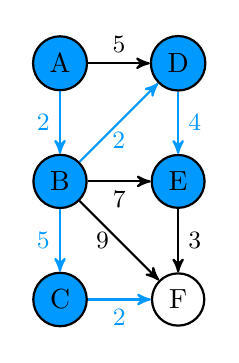
\begin{tikzpicture}[->,>=stealth',auto,node distance=1.5cm,
 thick,main node/.style={circle,draw}]
\node[main node,fill=blue!40!cyan](A)[]{A};
 \node[main node,fill=blue!40!cyan](D)[right of = A]{D};
 \foreach \s/\t in {B/A, C/B, E/D}{ 
     \node[main node, fill=blue!40!cyan](\s)[below of = \t]{\s};}
 \foreach \s/\t in {F/E}{ 
     \node[main node](\s)[below of = \t]{\s};}

 \path[every node/.style={font=\small},blue!40!cyan]
   (A) edge node[left]{2} (B)
    (B) edge node[below]{2} (D)
         
         edge node[left]{5} (C)
    (D) edge node{4} (E)
    (C) edge node[below]{2} (F);
  \path[every node/.style={font=\small}]
    (A) edge node{5} (D)
    (B) edge node[below]{7} (E)
          edge node [left]{9} (F)
    (E) edge node{3} (F);
    

 \end{tikzpicture}
 \end{center}
\end{columns}

\end{frame}
%-----------------------------------------------------
\begin{frame}
\frametitle{Dijkstra Example}

\begin{columns}[c]
\column{.5\textwidth}
\[
\begin{tabular}{|c|c|c|c|c|c|}
\hline
A*&B*&C*&D*&E*&F* \\
\hline
0& ~&~ &~ &~&~\\
\hline
0&2&~ &5&~&~\\
\hline
0&2&7&4&9&11\\
\hline
0& 2&7&4&8&11\\
\hline
0& 2&7&4&8&9\\
\hline
0& 2&7&4&8&9\\
\hline
0& 2&7&4&8&9\\
\hline
\end{tabular}
\]

\begin{itemize}
\item Add the node with the shortest distance
\end{itemize}

\column{.5\textwidth}
\begin{center}
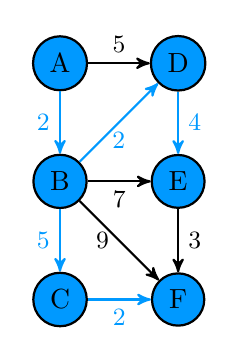
\begin{tikzpicture}[->,>=stealth',auto,node distance=1.5cm,
 thick,main node/.style={circle,draw}]
\node[main node,fill=blue!40!cyan](A)[]{A};
 \node[main node,fill=blue!40!cyan](D)[right of = A]{D};
 \foreach \s/\t in {B/A, C/B, E/D, F/E}{ 
     \node[main node, fill=blue!40!cyan](\s)[below of = \t]{\s};}

 \path[every node/.style={font=\small},blue!40!cyan]
   (A) edge node[left]{2} (B)
    (B) edge node[below]{2} (D)
         
         edge node[left]{5} (C)
    (D) edge node{4} (E)
    (C) edge node[below]{2} (F);
  \path[every node/.style={font=\small}]
    (A) edge node{5} (D)
    (B) edge node[below]{7} (E)
          edge node [left]{9} (F)
    (E) edge node{3} (F);
 \end{tikzpicture}
 \end{center}
\end{columns}

\end{frame}
%------------------------------------------------
\begin{frame}
\frametitle{Start at A, find the shortest path to each node}
\begin{columns}[c]
\column{.5\textwidth}
\[
\begin{tabular}{|c|c|c|c|c|c|}
\hline
A\only<2->{*}&B\only<8->{*}&C\only<12->{*}&D\only<6->{*}&E\only<4->{*}&F\only<10->{*}\\
\hline
\only<2->{0}& ~&~ &~ &~&~\\
\hline
\only<3->{0}&\only<3->{5}&~ &\only<3->{4}&\only<3->{1}&~\\
\hline
\only<4->{0}&\only<5->{5}&~&\only<5->{3}&\only<4->{1}&\only<5->{11}\\
\hline
\only<6->{0}&\only<7->{5}&~&\only<6->{3}&\only<6->{1}&\only<7->{11}\\
\hline
\only<8->{0}&\only<8->{5}&\only<9->{11}&\only<8->{3}&\only<8->{1}&\only<9->{7}\\
\hline
\only<10->{0}& \only<10->{5}&~\only<11->{10}&\only<10->{3}&\only<10->{1}&\only<10->{7}\\
\hline
\end{tabular}
\]
\column{.5\textwidth}

\begin{center}

\begin{tikzpicture}[auto,node distance=1.5cm,
 thick,main node/.style={circle,draw}]
\only<1>{\node[main node](A)[]{A};}
\only<2->{\node[main node,fill=blue!40!cyan](A)[]{A};}

\only<1-5>{\node[main node](D)[below of=A]{D};}
\only<6->{\node[main node,fill=blue!40!cyan](D)[below of=A]{D};}

\only<1-7>{\node[main node](B)[right of=A]{B};}
\only<8->{\node[main node,fill=blue!40!cyan](B)[right of=A]{B};}

\only<1-11>{\node[main node](C)[right of=B]{C};}
\only<12->{\node[main node,fill=blue!40!cyan](C)[right of=B]{C};}

\only<1-3>{\node[main node](E)[right of=D]{E};}
\only<4->{\node[main node,fill=blue!40!cyan](E)[right of=D]{E};}

\only<1-9>{\node[main node](F)[right of=E]{F};}
\only<10->{\node[main node,fill=blue!40!cyan](F)[right of=E]{F};}

    
\only<1-2>{\path[draw](A) edge node{5}(B);}
\only<3->{\path[draw, blue!40!cyan](A) edge node{5}(B);}

\only<1-2>{\path[draw](A) edge node{1}(E);}
\only<3->{\path[draw, blue!40!cyan](A) edge node{1}(E);}

\path[draw](B) edge node{8}(E);

\only<1-8>{\path[draw](B) edge node{2}(F);}
\only<9->{\path[draw, blue!40!cyan](B) edge node{2}(F);}

\only<1-8,11->{\path[draw](B) edge node{6}(C);}
\only<9-10>{\path[draw, blue!40!cyan](B) edge node{6}(C);}

\only<1-10>{\path[draw](C) edge node{3}(F);}
\only<11->{\path[draw, blue!40!cyan](C) edge node{3}(F);}

\only<1-4>{\path[draw](E) edge node[below]{2}(D);}
\only<5->{\path[draw, blue!40!cyan](E) edge node[below]{2}(D);}

\only<1-4,9->{\path[draw](E) edge node[below]{10}(F);}
\only<5-8>{\path[draw, blue!40!cyan](E) edge node[below]{10}(F);}

\only<1-2,5->{\path[draw](A) edge node[left]{4}(D);}
\only<3-4>{\path[draw, blue!40!cyan](A) edge node[left]{4}(D);}

\end{tikzpicture}

\end{center}

\end{columns}
\begin{center}
\only<2,4,6,8,10,12>{Add a node}
\only<3,5,7,9,11>{Update distances}
\end{center}
\end{frame}
%----------------------------------------------------

%%%%%%%%%%%% Coding %%%%%%%%%%%%%%%%%%%%%
%-----------------------------------------------------
\begin{frame}
\frametitle{Intoduction to Coding}
\begin{itemize}
\item \textbf{Coding} is the process of bijectively mapping a source alphabet  $S = \{s_1, s_2, ..., s_q\} $ into a set $C$ of codewords formed by combining strings from a code alphabet $A = \{ a_1, a_2, ..., a_p \}$.
\end{itemize}
\end{frame}
%-----------------------------------------------------
\begin{frame}
\frametitle{Coding Example}
\begin{itemize}
\item $S = \{ a, b,c, d, ..., z \}$
\item codewords $ = \{ 00, 01, 02, ..., 25\}$
\item $A = \{0,1,2,...,9\} $
\item The bijective mapping is $ a \mapsto 00, b \mapsto 01 , ..., z \mapsto 25$.
\item Then ACME $\mapsto 00021204$ .
\end{itemize}

\end{frame}
%-----------------------------------------------------
\begin{frame}
\frametitle{Vocabulary}
\begin{itemize}
\item The two digit numbers preserved \textbf{unique deciphering}.
\item If $C = \{1, 2, 3, ..., 25 \}$ then 
	\begin{itemize}
	\item rat $\mapsto 17019$ and 
	\item bhabj $\mapsto 17019$ 
	\end{itemize}
\item Keeping the two digits numbers means that words map uniquely.
\end{itemize}
\end{frame}
%-----------------------------------------------------
\begin{frame}
\frametitle{Vocabulary}
\begin{itemize}
\item A code is \textbf{instantaneous} if no codeword is a prefix of any other codeword.
	\begin{itemize}
	\item $C_1 = \{0, 01\} $ $0$ is a prefix of $01$.
	\item $C_2 = \{00, 01\} $ is an instantaneous code.
	\end{itemize}
\item Instantaneous codes are easier to decipher because we know right away where a word ends.
\end{itemize}
\end{frame}
%-----------------------------------------------------
\begin{frame}
\frametitle{Vocabulary}
\begin{itemize}
\item An \textbf{information scheme} is an ordered pair $(S,P)$ where $S$ is the source alphabet and $P$ is a probability distribution.
\item $P(s_i)$ is the probability of $s_i$ where $s_i \in S$.
\item An \textbf{encoding scheme} is an ordered pair $(C,f)$ where $C$ is the set of codewords and $f: S \rightarrow C$. 
\end{itemize}
\end{frame}
%----------------------------------------------------
\begin{frame}
\frametitle{Coding Example}
\begin{itemize}
\item $S = \{a, b, c, d\}$
\item $P(a) = \frac{2}{17}, P(b) = \frac{2}{17}, P(c) = \frac{8}{17}, P(d) = \frac{5}{17}$
\pause
\item Scheme A: $a \mapsto 11, b \mapsto 0, c \mapsto 100, d \mapsto 1010$
\item Scheme B: $a \mapsto 01011, b \mapsto 00, c \mapsto 10, d \mapsto 11$
\end{itemize}
\pause
\begin{columns}[c]
\column{.5\textwidth}
\begin{center}
Scheme A
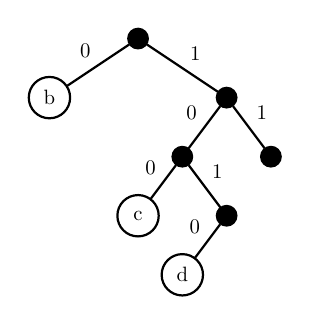
\begin{tikzpicture}[scale = .75, transform shape, auto,thick, main node/.style={circle, draw, minimum size=.7cm}, dot node/.style={circle, draw, fill=black}, level distance=1cm, 
    level 1/.style={sibling distance=3cm}, level 2/.style={sibling distance=1.5cm}]
\node[dot node]{}
    child{node[main node]{b}
        edge from parent node[above left]{0}
    }
    child{node[dot node]{}
        child{node[dot node]{}
            child{node[main node]{c}
                edge from parent node[above left]{0}}
            child{node[dot node]{}
                child{node[main node]{d}
                    edge from parent node[above left]{0}}
                child[fill=none] {edge from parent[draw=none]}
                edge from parent node{1}          
            }
            edge from parent node[above left]{0}
        }
        child{node[dot node]{}
            edge from parent node{1}}
        edge from parent node{1}
    };
\end{tikzpicture}
\end{center}
\column{.5\textwidth}
\begin{center}
Scheme B
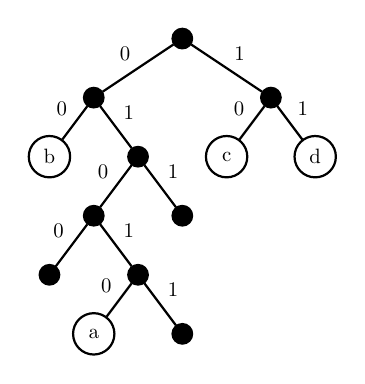
\begin{tikzpicture}[scale = .75, transform shape, auto,thick, main node/.style={circle, draw, minimum size=.7cm}, dot node/.style={circle, draw, fill=black}, level distance=1cm, 
    level 1/.style={sibling distance=3cm}, level 2/.style={sibling distance=1.5cm}]
\node[dot node]{}
    child{node[dot node]{}
        child{node[main node]{b}
            edge from parent node[above left]{0}}
        child{node[dot node]{}
            child{node[dot node]{}
                child{node[dot node]{}
                    edge from parent node[above left]{0}}
                child{node[dot node]{}
                    child{node[main node]{a}
                        edge from parent node[above left]{0}}
                    child{node[dot node]{}
                        edge from parent node{1}}
                    edge from parent node{1}
                }
                edge from parent node[above left]{0}
            }
            child{node[dot node]{}
                edge from parent node{1}}
            edge from parent node{1}
        }
    edge from parent node[above left]{0}
    }
    child{node[dot node]{}
        child{node[main node]{c}
            edge from parent node[above left]{0}}
        child{node[main node]{d}
            edge from parent node{1}}
    edge from parent node{1}
    };
\end{tikzpicture}
\end{center}

\end{columns}
\end{frame}
%-------------------------------------------------------
\begin{frame}
\frametitle{Coding Example}
\begin{itemize}
\item What is the average codeword length?
\item Ave $= \sum_{i=1}^{n} len(f(s_i))p(s_i)$ 
\item Scheme A: $ 2*\frac{2}{17} + 1*\frac{2}{17} + 3*\frac{8}{17} + 4*\frac{5}{17} = \frac{50}{17}$
\item Scheme B: $ 5*\frac{2}{17} + 2*\frac{2}{17} + 2*\frac{8}{17} + 2*\frac{5}{17} = \frac{40}{17}$
\end{itemize}

\end{frame}
%----------------------------------------------------
\begin{frame}
\frametitle{Coding Example}
\begin{itemize}
\item Scheme B is shorter to use on average despite having a codeword that is 5 characters long. 
\item $a$ has a much lower probability than $c$ or $d$.
\item This means less data to send and to work with.
\item Even though both codes are uniquely decipherable and instantaneous, scheme B would usually be the better one to use.
\end{itemize}
\end{frame}
%------------------------------------------------------
%Huffman encoding
\begin{frame}
\frametitle{Huffman Encoding}
\begin{itemize}
\item An ideal encoding scheme will have a low average word length.
\item Words with higher probabilitiesl have a shorter codewords
\item Rarer words have a longer codewords.
\item \textbf{Huffman encoding} is an algorithm for creating a code with optimized average codeword length.
\item Also is uniquely deciperable and instataneaous

\end{itemize}
\end{frame}

%----------------------------------------------------
\begin{frame}
\frametitle{Huffman Example}
\begin{columns}[c]
\column{.5\textwidth}
\begin{itemize}
\item Same source alphabet as before.
\item $c$ has the highest probability and the shortest codeword.
\item $a$ and $b$ have the lowest probabilities and the longest codewords.
\item Average codeword length $= \frac{30}{17}$
\end{itemize}
\column{.5\textwidth}
\begin{center}
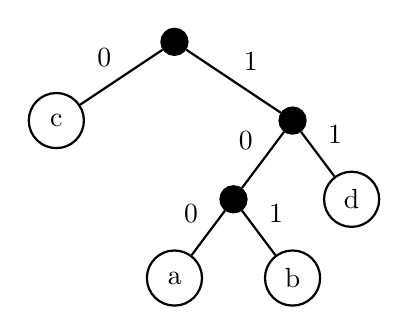
\begin{tikzpicture}[auto,thick, main node/.style={circle, draw, minimum size=.7cm}, dot node/.style={circle, draw, fill=black}, level distance=1cm, 
    level 1/.style={sibling distance=3cm}, level 2/.style={sibling distance=1.5cm}]
\node[dot node]{}
    child{node[main node]{c}
        edge from parent node[above left]{0}
    }
    child{node[dot node]{}
        child{node[dot node]{}
            child{node[main node]{a}
                edge from parent node[above left]{0}}
            child{node[main node]{b}
                edge from parent node{1}}
            edge from parent node[above left]{0}
        }
        child{node[main node]{d}
            edge from parent node{1}}
        edge from parent node{1}
    };
\end{tikzpicture}
\end{center}
\end{columns}

\end{frame}
%----------------------------------------------------
\begin{frame}
\frametitle{Huffman Algorithm}
\begin{itemize}
\item Sort words by probabilities from least to greatest.
\item Combine the two least words into a tree.
\item Repeat until everything is in the tree.

\end{itemize}

\end{frame}
%----------------------------------------------------
\begin{frame}
\frametitle{Huffman Example}
\begin{columns}[c]
\column{.3\textwidth}
\[
\begin{tabular}{|c|c|}
\hline
Symbol & Prob \\
\hline
a & 0.35 \\
b & 0.10 \\
c & 0.19 \\
d & 0.25 \\
1 & 0.06 \\
2 & 0.05 \\
\hline
\end{tabular}
\]
\column{.7\textwidth}
\begin{center}
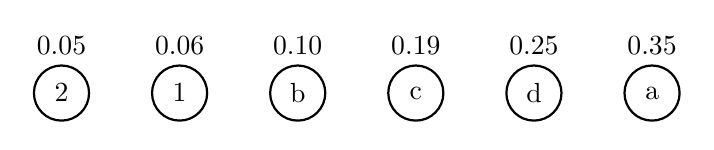
\begin{tikzpicture}[auto, node distance=1.5cm, thick, main node/.style={circle, draw, minimum size=.7cm}]% Minimum size adjusted to compensate for the c
\node[main node](2)[]{2};
\foreach \s/\t in {1/2, b/1, c/b, d/c, a/d}{
    \node[main node] (\s) [right of = \t] {\s};}
\tikzset{node distance = .6cm}
\foreach \s/\t in {2/0.05, 1/0.06, b/0.10, c/0.19, d/0.25, a/0.35}{
    \node[draw=none] (\t) [above of = \s]{\t};} 
\end{tikzpicture}   
\end{center}
\end{columns}
\end{frame}
%----------------------------------------------------
\begin{frame}
\frametitle{Huffman Example}

\begin{center}
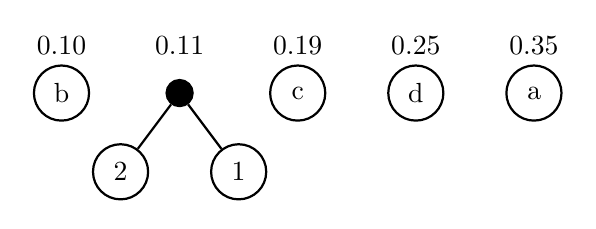
\begin{tikzpicture}[auto, node distance=1.5cm, thick, main node/.style={circle, draw, minimum size=.7cm}, level distance=1cm]
\node[draw=none](0.10)[]{0.10};
\foreach \s/\t in {0.11/0.10, 0.19/0.11, 0.25/0.19, 0.35/0.25}{
    \node[draw=none] (\s) [right of = \t] {\s};}
\node[circle, draw, fill=black, node distance=.6cm](dot)[below of = 0.11]{}
    child {node[main node]{2}}
    child {node[main node]{1}};
\tikzset{node distance = .6cm}
\foreach \s/\t in {b/0.10, c/0.19, d/0.25, a/0.35}{
    \node[main node] (\s) [below of = \t] {\s};}
\end{tikzpicture}
\end{center}

\end{frame}
%----------------------------------------------------
\begin{frame}
\frametitle{Huffman Example}

\begin{center}
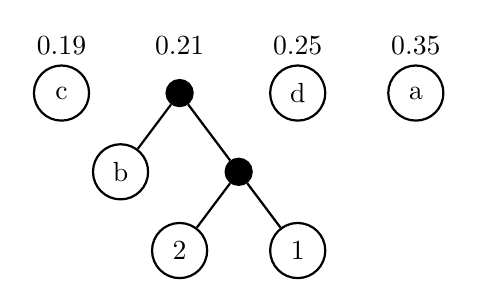
\begin{tikzpicture}[auto, node distance=1.5cm, thick, main node/.style={circle, draw, minimum size=.7cm}, dot node/.style={circle, draw, fill=black}, level distance=1cm]
\node[draw=none](0.19)[]{0.19};
\foreach \s/\t in {0.21/0.19, 0.25/0.21, 0.35/0.25}{
    \node[draw=none] (\s) [right of = \t] {\s};}
\node[dot node, node distance=.6cm](dot)[below of = 0.21]{}
    child {node[main node]{b}}
    child {node[dot node]{}
        child {node[main node]{2}}
        child {node[main node]{1}}
    };
\tikzset{node distance = .6cm}
\foreach \s/\t in { c/0.19, d/0.25, a/0.35}{
    \node[main node] (\s) [below of = \t] {\s};}
\end{tikzpicture}
\end{center}

\end{frame}
%----------------------------------------------------
\begin{frame}
\frametitle{Huffman Example}

\begin{center}
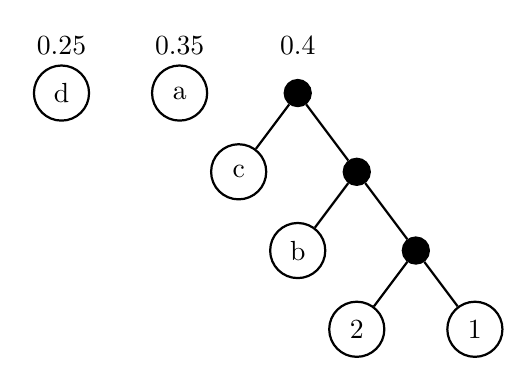
\begin{tikzpicture}[auto, node distance=1.5cm, thick, main node/.style={circle, draw, minimum size=.7cm}, dot node/.style={circle, draw, fill=black}, level distance=1cm]
\node[draw=none](0.25)[]{0.25};
\node[draw=none](0.35)[right of=0.25]{0.35};
\node[draw=none](0.4)[right of=0.35]{0.4};
\node[dot node, node distance=.6cm](dot)[below of = 0.4]{}
    child {node[main node]{c}}
    child {node[dot node]{}
        child {node[main node]{b}}
        child {node[dot node]{}
            child {node[main node]{2}}
            child {node[main node]{1}}
        }
    };
\tikzset{node distance = .6cm}
\foreach \s/\t in {d/0.25, a/0.35}{
    \node[main node] (\s) [below of = \t] {\s};}
\end{tikzpicture}
\end{center}

\end{frame}
%----------------------------------------------------
\begin{frame}
\frametitle{Huffman Example}

\begin{center}
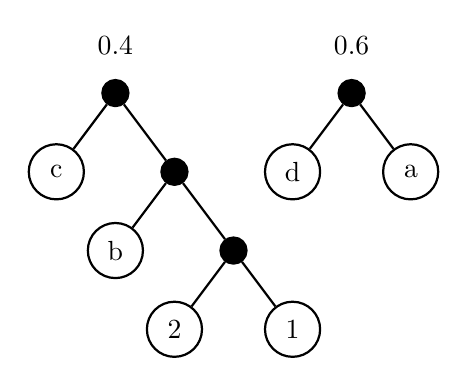
\begin{tikzpicture}[auto, node distance=3cm, thick, main node/.style={circle, draw, minimum size=.7cm}, dot node/.style={circle, draw, fill=black}, level distance=1cm] %Node distance adjusted to 3cm to allow enough room for both parts of the step
\node[draw=none](0.4)[]{0.4};
\node[draw=none](0.6)[right of=0.4]{0.6};
\node[dot node, node distance=.6cm](dot)[below of = 0.4]{}
    child {node[main node]{c}}
    child {node[dot node]{}
        child {node[main node]{b}}
        child {node[dot node]{}
            child {node[main node]{2}}
            child {node[main node]{1}}
        }
    };
\node[dot node, node distance=.6cm][below of = 0.6]{}
    child {node[main node]{d}}
    child {node[main node]{a}};
\end{tikzpicture}
\end{center}

\end{frame}
%----------------------------------------------------
\begin{frame}
\frametitle{Huffman Example}

\begin{center}
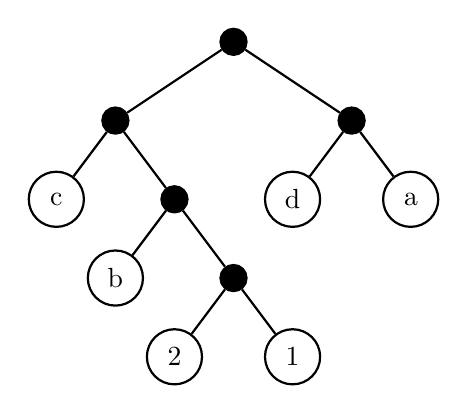
\begin{tikzpicture}[auto,thick, main node/.style={circle, draw, minimum size=.7cm}, dot node/.style={circle, draw, fill=black}, level distance=1cm, 
    level 1/.style={sibling distance=3cm}, level 2/.style={sibling distance=1.5cm}]
\node[dot node]{}
    child{node[dot node]{}
        child{node[main node]{c}}
        child{node[dot node]{}
            child{node[main node]{b}}
            child{node[dot node]{}
                child{node[main node]{2}}
                child{node[main node]{1}}
            }
        }
    }
    child{node[dot node]{}
        child{node[main node]{d}}
        child{node[main node]{a}}
    };
\end{tikzpicture}
\end{center}

\end{frame}
%----------------------------------------------------
\end{document}


\end{document}